\section{Related Work}\label{sec:Background}

Most work on push manipulation in robots
\cite{mason_manipulator_1982,lynch_mechanics_1992,peshkin_motion_1988,cappelleri_designing_2006}
it is restricted to planar sliding motions of what are effectively 2D
objects. Little work addresses push manipulation on real 3D bodies,
which are free to tip or roll. Rigid body simulators are used for
prediction, but rely on explicit knowledge of parameters which are
difficult to ascertain. Even then, such predictions may not be
possible due to inherent limitations of the physical model employed,
for example when modelling
friction.% \cite{mason_mechanics_2001}. %Once a physics simulator has been set up for a particular scenario, it is not generalisable to new objects or novel situations~\cite{cappelleri_designing_2006}.

Some machine learning approaches have been developed to classify or
provide predictions for objects or object classes, e.g. rolling versus
non-rolling objects
\cite{fitzpatrick_learning_2003,ridge_towards_2008}, or liftable
versus non-liftable objects \cite{paletta_learning_2007}. These works
are limited, in that predictions learned may not be generalisable to a
new object, pose or push direction, and explicit 6-DoF rigid body
motions are not predicted. In contrast, our approach predicts explicit
rigid body transformations, and generalisation to novel push
directions, object poses, and shapes.

\begin{figure}[t]
%\centerline{\includegraphics[width=\the\barchartwidth]{graphs_jw/S1_sim_av_graph}}
\centerline{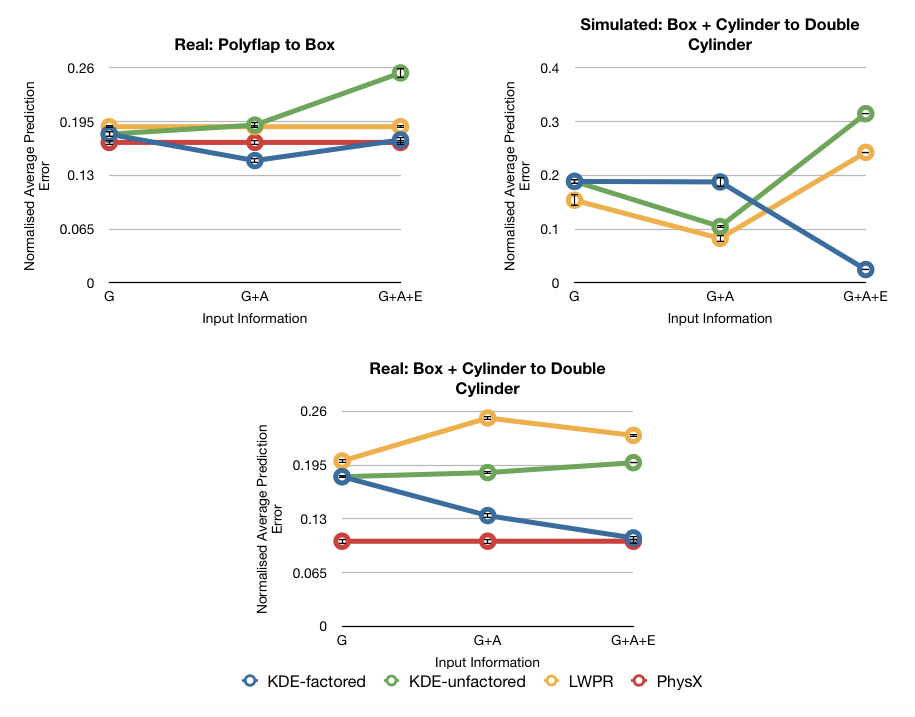
\includegraphics[width=0.95\columnwidth]{graphs_jw/S_real_sim_av_graph}
%\centerline{\includegraphics[width=0.45\columnwidth]{graphs_jw/S1_real_av_graph.png}
%\includegraphics[width=0.45\columnwidth]{graphs_jw/S2_real_av_graph}}
%\centerline{\includegraphics[width=0.45\columnwidth]{graphs_jw/S2_sim_av_graph}
%\includegraphics[width=0.45\columnwidth]{graphs_jw/S3_sim_av_graph.png}
}
\centerline{
\includegraphics[width=0.9\columnwidth]{graphs_jw/graph_key}}
\caption{Experiment P3: Comparative performance of predictors vs. information utilised, as measured by the normalised average error ${E_{av}^{norm}}$. 
}\label{fig:S_av_graphs}
\end{figure}

%One of the issues explored in this paper is how a combination of appropriately
%trained factored probability density can facilitate a degree of generalisation
%with respect to making predictions about objects with different shapes
%or subjected to different manipulative actions
%than those encountered during training.
%Other researchers have also looked at various ways of combining
%the output of multiple predictors,
%in the context of machine learning approaches to motor control.
%Work from the computational neuroscience literature \cite{Haruno_MOSAIC_2008},
%suggests a continuously re-learnable model for modular motor control,
%where complex control signals can be created from a weighted combination
%of the outputs of a set of learned forward models,
%each of which is itself comparatively simple.
%The forward models may be thought of as corresponding to
%predictors for different contexts.
%The work is demonstrated through a simple simulation experiment,
%and is shown to exhibit a degree of interpolative generalisation.
%in which the learned controllers are applied to a 1D mass-spring-damper system
%where the three key system parameters can adopt different values.
%A degree of interpolative generalisation is shown,
%e.g. two modules that are trained for large mass and small mass can
%combine their outputs to effectively control a medium-sized mass. 

Stoytchev \cite{Stoytchev_affordances_2008} described a robotic system
that learns affordances of sticks and hook-like tools by using them to
push observed objects.  A relationship is learned between an action
with a particular tool, and the resulting motion of the pushed
object. This work feaured 2D scenes, in which the motions of
puck-like discs were restricted to a plane, under four discrete
possible actions.
%very simple objects (puck-like discs) were restricted to sliding on a 2D table-top,
%under only four discrete possible actions
%(pushing away from or towards the robot, and in left and right directions).
Importantly, while the outcomes of actions could be learned for tools
of various shapes, the system was not able to apply knowledge
learned from one tool to make predictions about another tool of similar shape.
%For example, the behaviours of two different tools that both share
%a hook-shaped section must be learned separately for each tool -- the
%system cannot apply knowledge about the influence of hook-shape,
%learned while exploring one tool,
%to make predictions about a new tool that shares the same shape.
%In contrast, in this paper we present a method by which knowledge about the
%behaviour of one pushed object can be transferred to
%another object which has a different shape.
%This is because small component parts of each object may share
%commonalities which may influence the objects' behaviours in common ways --
%by decomposing objects into local parts, and assigning independent
%predictive factors to each, we show how a learning system with a
%degree of shape generalisation is possible.
%In contrast, in this paper we show how a learning system with a
%degree of action and shape generalisation is possible, 
%by decomposing objects into local parts, and assigning independent
%predictive factors to each.

%\begin{table}[b]
%\begin{center}
%\begin{tabular}{|l|l|l|l|l|}
%\cline{3-5}
%\multicolumn{2}{c}{ } & \multicolumn{3}{|c|}{Information Utilised} \\
%\cline{1-5}
%Predictor & data & Global\,(G) & G\,\&\,Agent\,(A) & G\,\&\,A\,\&\,Env \\
%\cline{1-5}
%%KDEF & sim & 0.167 & n/a & \textbf{0.111} \\
%%LWPR & sim & 0.118 & n/a & n/a \\
%%\cline{1-5}
%KDEF & real & 0.180$\pm$0.004 & \textbf{0.148}$\pm$0.003 & 0.173$\pm$0.004 \\
%LWPR & real & 0.189$\pm$0.002 & 0.189$\pm$0.002 & 0.189$\pm$0.002 \\
%KDE & real & n/a & 0.191 $\pm$ 0.004 & 0.254 $\pm$ 0.006 \\
%\cline{3-5}
%PhysX & real & \multicolumn{3}{|c|}{0.170 $\pm$ 0.003} \\
%\cline{1-5}
%\end{tabular}
%\end{center}
%\caption[Performance Table]{Experiment S-transfer: Generalisation to novel shape.
%Trained on polyflap, tested on box, for real data.
%Comparative performance of predictors vs. information used.
%Shown is the dimensionless measure normalised average error ${E_{av}^{norm}} \pm$ standard error.
%}\label{tab:PerformanceTableS1av}
%\end{table}

